\documentclass[a4paper,10pt]{article}
%\usepackage[utf8x]{inputenc}
\usepackage{amsmath}
\usepackage[pdftex]{graphicx}
%opening
\title{Programing Techniques for Scientific Simulations: Report B}
\author{Marion Baumgartner}

\begin{document}

\maketitle

\section{Simpson Integration}

Simpson's rule is used to integrate several different function such as 
\begin{align*}
f(x)&=1\\
f(x)&=x\\
f(x)&=x^2\\
f(x)&=\sin(x)\\
f(x)&=\sin(5\cdot x)
\end{align*}
The functions are all integrated in an interval $[0,\pi]$ using $N=100$ steps. The basic formula used is

\begin{align}
\label{simpson}
    Q(f)=\frac{h}{3} \cdot \left( \frac {1}{2} f(x_0)+\sum_{k=1}^{N-1}f(x_k)+2\sum_{k=1}^{N}f \left( \frac{x_{k-1}+x_k}{2} \right)+\frac{1}{2} f(x_N) \right)\\
    h=\frac{b-a}{N} \hspace{3cm} x_k=a+k\cdot h\nonumber
\end{align}

Where $[a,b]$ is the interval to be integrated over and $N$ determines the number of bins ($N$ has to be even). Further we have that
\begin{align}
  \int_{a}^{b}f(x)dx=Q(f).
\end{align}


I used several different methods to program the algorithm of the Simpson function. These were
\begin{enumerate}
\item Hard-Core function
\item function pointers
\item (template) function objects
\item virtual functions
\end{enumerate}
The Run times of the different methods with the different functions are shown in table \ref{tabel1} and they are graphically presented in figure \ref{fig4}.



\begin{table}
\centering
  \begin{tabular}{|c|c|c|c|c|c|c|} \hline
f(x)&	1&	$x$&	$x^2$&	$\sin(x)$&	$\sin(5\cdot x)$\\ \hline\hline
Hard-Core function&		4	&5	&7.15	&9	&28\\ \hline
function pointers		&9.1	&12.9	&14	&44	&45 \\ \hline
function objects		&10	&5.69	&6.16	&28	&22 \\ \hline
virtual functions		&35	&39	&42.2	&28.8	&30 \\ \hline
  \end{tabular}
  \caption{Run times of the programs. All the times are given in $10^{-6}$sec.}
  \label{tabel1}
\end{table}

As we can see from the table for the functions given the fastest is the hard-cored function method. The slowest program for simple function such as $f(x)=1; \; f(x)=x;$ and $f(x)=x^2$ is the one done with virtual functions. For more complex functions ($f(x)=\sin(x)$ and $f(x)=\sin5(x)$) the program  using function pointer is the slowest. 
the reason why the program using virtual functions is slow is because the polymorphic function resolution occurs at runtime and indirect virtual functions tables calls are made only at runtime. This causes time to be similar for all functions $f(x)$.
An Improvement in the program using Hard-Core function and function pointers could perhaps e achieved by inlining the function call of $f(x)$

\begin{figure}[h]
\centering
 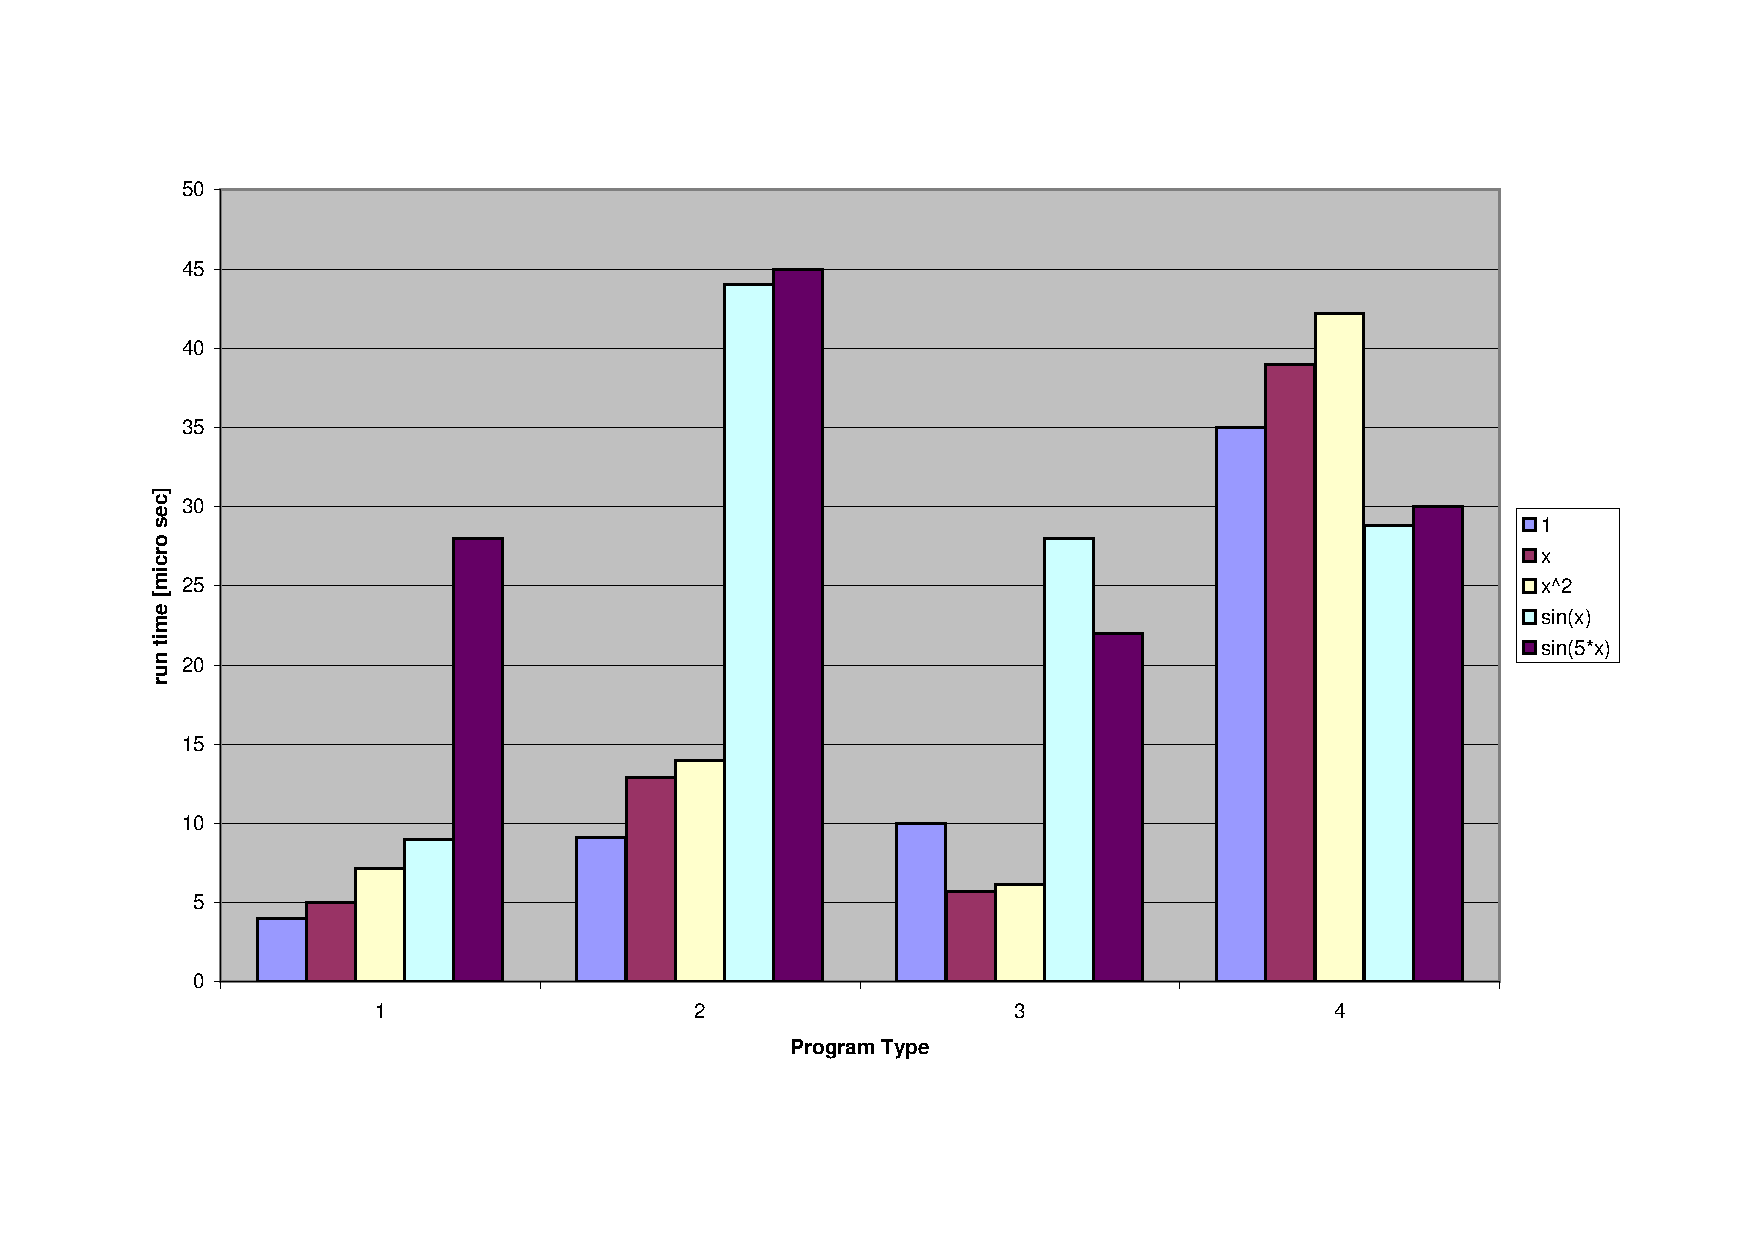
\includegraphics[viewport=60pt 70pt 800pt 500pt, clip, width=\textwidth]{Graph}
 \caption{run time of the different implementations of the Simpson method. Method 1 is the Hard-Core function method; 2 is the version using function pointers; 3 uses  (template) function objects and 4 is programed with virtual functions. }
\label{fig4}
\end{figure}
\end{document}
